\documentclass[]{article}
\usepackage{graphicx}
%\graphicspath{ {images/} }
\usepackage{wrapfig}
\usepackage{enumerate}
\usepackage{natbib}
\usepackage{url}
\usepackage{amsfonts}
\usepackage{mathtools}

\newcommand{\ZZ}{\ensuremath{\mathbb{Z}}}
%opening
\title{CHVote: Efficient modular exponentiations}
\author{Nicolas GAILLY}

\begin{document}

\maketitle

\section{Introduction} \label{intro}

The canton of Geneva is working on a new digital votation system called
CHVote \cite{chvote} whose main goal is to increase the electorate confidence 
by providing a secure, transparent and usable online voting system. The final
product must enable a Swiss citizen to vote on any election mandated by the
Geneva canton using his laptop or mobile phone in a browser environment.

In this work, we focus on the vote casting part of the system from the client
side. In order to cast a vote, the client has to perform an k-out-of-n oblivious
transfer protocol \cite{chu2005} with the votation servers. In this protocol,
the client must perform between a few and a hundred of modular exponentiation
computation, depending on the number of votes the client has to perform for a
particular votation. In the context of CHVote, these modular exponentiation
computations take place in a multiplicative group whose order is a large prime
$q$. It is typically expected for security reason in this scenario that the number
of bits needed to represent q can lie between 1024 bits and up to 8192 bits.

The potentially large number of computation on the client side is problematic in
this context.  Indeed, modular exponentiation with a large modulo is a
computationally expensive operation. Typical optimization in this space has been
to provide hand written assembly code such as the GMP library \cite{gmplib}
coded in a mix of C and assembly. Unfortunately, such code is not able to run in
a browser environment. Therefore, the client typically has to rely on
Javascript, an interpreted language ran in the browser context to perform these
operations.  Unfortunately, Javascript performs quite poorly for such extensive
computations \cite{jsbad}.

In this work, we present an efficient way of computing these modular
exponentation relying on multiple third party servers. This work presents our solution
in section \ref{design}, our evaluation in section \ref{evaluation}, and finally some open
questions to be addressed in section \ref{discussions}.

\section{Design} \label{design}

The goal of the project is to find an efficient scheme for the client to perform
modular exponentiations. In the context of CHVote, the client only must know
about the exponent; the base and the modulo need not to be private, simplifying
significantly the design of the solution.

We assume we are working in a multiplicative group $G$ of order prime $q$. We denote
the base $b \in \ZZ_q^*$ and the exponent $a \in \ZZ_q^*$. We want to find an
efficient way to compute: $$ b^a \mod q $$

The core idea is to decentralize the computation to third party servers while
keeping the exponent secret by using a trivial non-threshold secret sharing
scheme. We suppose we want to use $n$ external servers to compute the modular
exponentiation. Formally, the secret sharing generates $n-1$ random values $r_i
\in \ZZ_q^*$ for $i=0...n-2$ and sets $r_{n-1} = {a - \sum_{i=0}^{n-2} r_i} \mod
q$

\section{Evaluation} \label{evaluation}

\begin{figure}[!htb]
    \begin{center}
        \label{fig:system}
        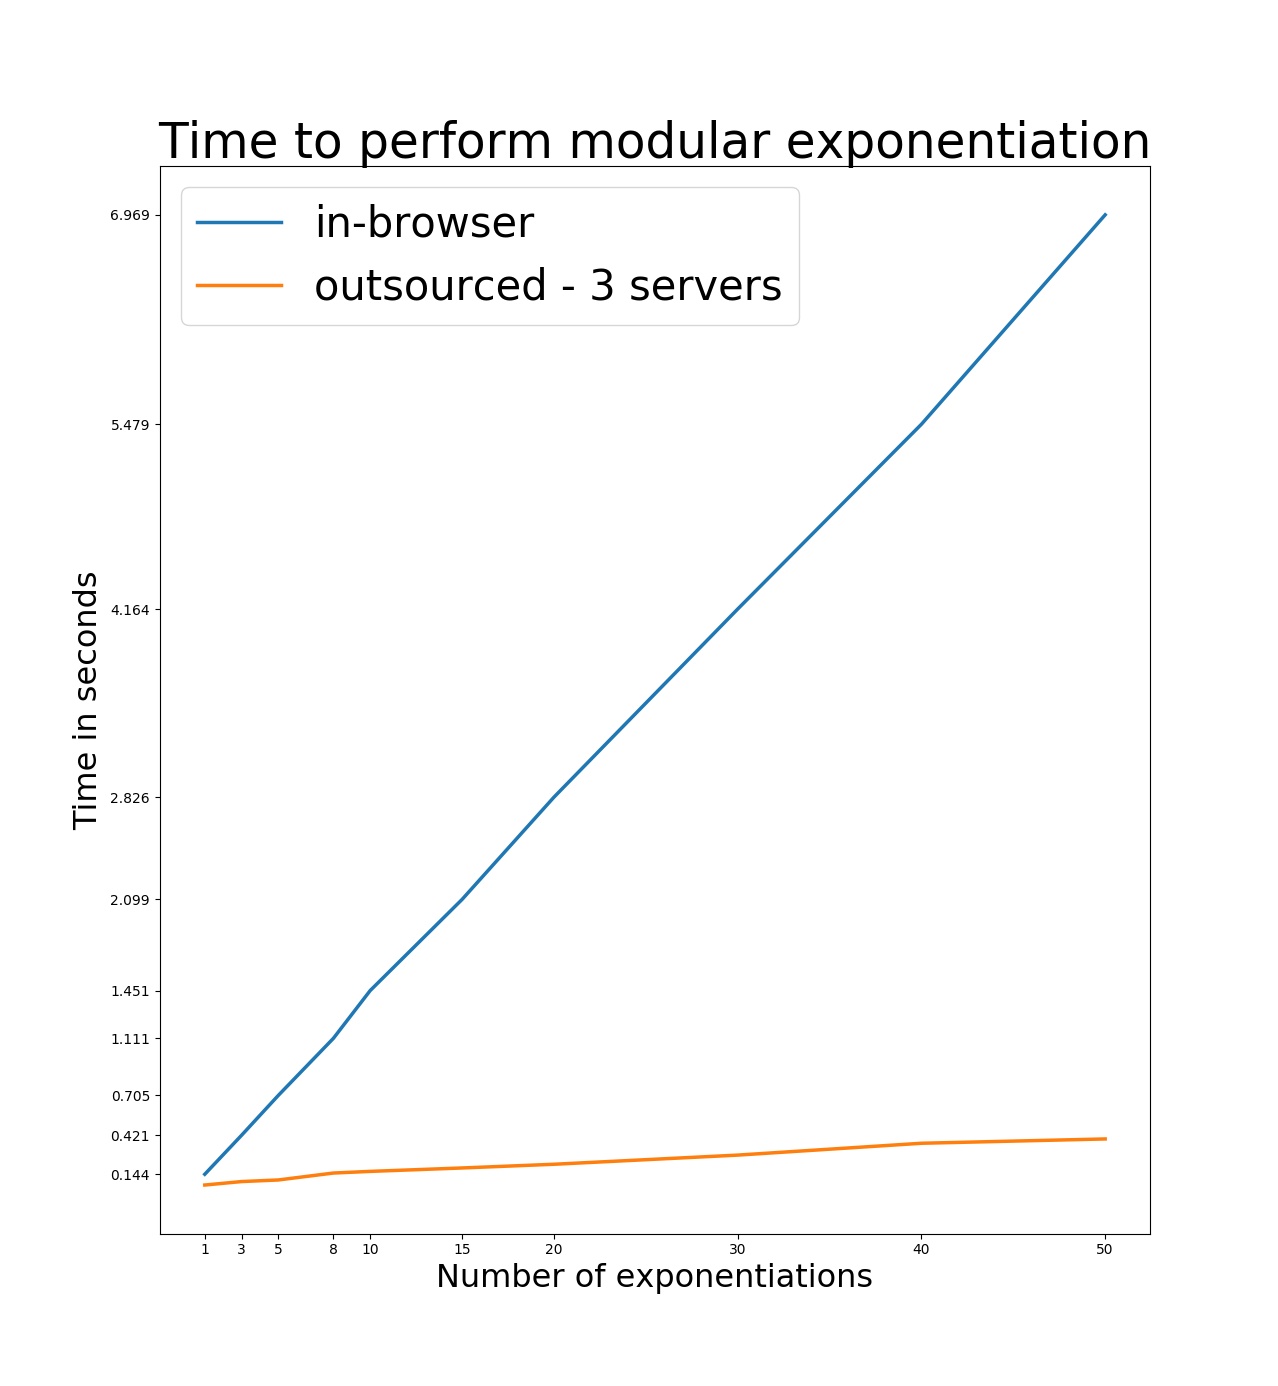
\includegraphics[trim={0 8cm 0
        1cm},clip,width=1.2\textwidth]{local_vs_split_50.png}
        \caption{\textbf{Performance of the in-browser computation vs
        outsourced computation}.}
    \end{center}
\end{figure}

\section{Discussions} \label{discussions}

\bibliographystyle{plain}
\bibliography{main}

\end{document}
